\documentclass[t]{beamer}
\usepackage{CJKutf8}
\usepackage{amsfonts}
    \usepackage{amsmath}
    \usepackage{amssymb}
    \usepackage{amsthm}
    \usepackage{enumerate}
    \usepackage{graphicx}
    \usepackage{layout}
    \usepackage{mathrsfs}
    \usepackage{fancyhdr}
    \usepackage{subfigure}
    \usepackage{tcolorbox}
    \usepackage{tikz-cd}
    \usepackage{color}
    \usepackage{pifont}
    \usepackage{verbatim}
    \usepackage{mathtools}
    \usepackage{float}
    \usepackage{bm}
    \usetheme{AnnArbor}
% \usetheme{Antibes}
\usecolortheme{beaver}
\usepackage{listings}

% 设置JSON样式
\lstdefinestyle{json}{
    basicstyle=\tiny\ttfamily,
    columns=fullflexible,
    showstringspaces=false,
    commentstyle=\color{gray},
    keywordstyle=\color{blue},
    stringstyle=\color{red},
    breaklines=true,
    frame=single,
    captionpos=b,
    aboveskip=10pt,
    belowskip=10pt
}

% 设置shell样式
\lstdefinestyle{shell}{
    language=bash,
    basicstyle=\tiny\ttfamily,
    columns=fullflexible,
    showstringspaces=false,
    commentstyle=\color{gray},
    keywordstyle=\color{blue},
    stringstyle=\color{red},
    breaklines=true,
    frame=single,
    captionpos=b,
    aboveskip=10pt,
    belowskip=10pt
}

% 添加网址的命令
\usepackage{hyperref}
% 这是一个带链接文本的示例:\href{https://www.example.com}{点击这里访问网站}
% 普通的示例:\url{https://www.example.com}
% 表格
\usepackage{booktabs}
\usepackage{multirow}

% \setbeamertemplate{navigation symbols}{}

\usepackage{textpos}

\newcommand{\dif}{\mathrm{d}}
\newtheorem{thm}{{定理}}

% some common command
\newcommand{\mm}[1]{$ #1$\newline}
% \newcommand{\tuichu}{\Rightarrow}
% \newcommand{\li}[1]{\newline#1}



\newcommand{\analysis}[2]{\forall \mathcal{E}{#1},\exists \delta {#2},s.t.}
\newcommand{\denyanalysis}[2]{\exists \mathcal{E}{#1},\forall \delta {#2},s.t.}
\newcommand{\yield}{\Rightarrow }
\newcommand{\jj}{\newline}
\newcommand{\ff}[1]{$ #1$}   % math environment + newline
\newcommand{\fgn}[1]{\begin{equation}#1\end{equation}  }
\newcommand{\fg}[1]{$$ #1$$}   % math environment + newline 
\newcommand{\pf}{$proof.$\newline}
\newcommand{\ee}{\newline\ff{\Box}\newline}
\newcommand{\fenshi}[2]{\ff{\frac{#1}{#2}}}
\newcommand{\shenlue}{\vdots\jj}
\newcommand{\abs}[1]{{\left \lvert #1 \right\rvert}}
\newcommand{\loge}[1]{In ({#1})}
\newcommand{\logical}[2]{log_{#2}^{#1}}
\newcommand{\summary}[3]{$\sum_{{#1}={#2}}^{#3}  $}
\newcommand{\denjia}[2]{{#1}\Leftrightarrow {#2}}
\newcommand{\jihe}[3]{ {#1}  = \{ {#2} \mid {#3} \} }
\newcommand{\ve}[2]{\left\langle {#1},{#2}\right \rangle}
\newcommand{\dakuohao}[2]{\begin{array}{rcl}{#1}\end{array} \} \Rightarrow{#2}}
\newcommand{\sxb}[3]{#1^{#2}_{#3}}
\newcommand{\sss}[2]{#1^{#2}}
\newcommand{\xxx}[2]{#1_{#2}}
\newcommand{\bri}[1]{\uppercase\expandafter{\romannumeral#1}}
\newcommand{\ri}[1]{\romannumeral#1} 
\newcommand{\polynomial}[8]{#1_{#2}#6^{#7}+#1_{#3}#6^{#8}+...+#1_{#4}#6+#1_{#5} }
\newcommand{\newd}[4]{f[{#1}_{#2},{#4},{#1}_{#3}]}
\newcommand{\lb}[2]{\begin{align*}\begin{split}{#1}\{ {#2}\end{split}\end{align*}}
\newcommand{\tab}[1]{\begin{array}{ll} {#1}\end{array}}


% 向量乘积
\newcommand{\avg}[1]{\left\langle #1 \right\rangle}
% 偏微分方程
\newcommand{\difFrac}[2]{\frac{\dif #1}{\dif #2}}
\newcommand{\pdfrac}[2]{\frac{\partial{#1}}{\partial{#2}}}
% 不同章节
\newcommand{\one}[1]{\section{#1}}
\newcommand{\two}[1]{\subsection{#1}}
\newcommand{\three}[1]{\subsubsection{#1}}
\newcommand{\aone}[1]{\section*{#1}}
\newcommand{\atwo}[1]{\subsection*{#1}}
\newcommand{\athree}[1]{\subsubsection*{#1}}
% 大括号,左右都有
\newcommand{\lbra}[1]{\left\{  {\begin{matrix} #1 \end{matrix}}\right. } 
% 样式 括号前缀 + 括号 
\newcommand{\lbras}[2]{{#1}\left\{ {  {\begin{matrix} #2 \end{matrix}}}\right. } 
\newcommand{\rbra}[1]{ \left.  {\begin{matrix} #1 \end{matrix}} \right\}  } 
% 模长
\newcommand{\distance}[1]{\parallel #1\parallel }
% 等价
\newcommand{\equ}{\Longleftrightarrow }
% 共轭
\newcommand{\cja}[1]{\overline{#1}}
% 两个矩阵,上面是 方框[] 下面是线条| 中间是 无
\newcommand{\mtx}[1]{\begin{matrix}#1\end{matrix} }
\newcommand{\bmtx}[1]{\begin{bmatrix}#1\end{bmatrix} }
\newcommand{\vmtx}[1]{\begin{vmatrix}#1\end{vmatrix} }
% \newcommand{\table}[1]{\begin{array}[lr]{ccc} #1 \end{array}}

%输入普通字符
\newcommand{\ww}[1]{\text{#1}}

% 所有内容 直接头文件搞定
\newcommand{\everything}[1]{\begin{document}\begin{CJK*}{UTF8}{gkai}#1\end{CJK*}\end{document}}


% 存放代码(失败了)
\newcommand{\cccode}[1]{\begin{lstlisting}#1\end{lstlisting}}

% 改变特定行序列
\newcommand{\ttt}{\subsection{}}

% 嵌套序号
\newcommand{\eee}[1]{\begin{enumerate}#1\end{enumerate}}


% 模板里面的一些宏
\newcommand{\pdfFrac}[2]{\frac{\partial #1}{\partial #2}}
\newcommand{\OFL}{\mathrm{OFL}}
\newcommand{\UFL}{\mathrm{UFL}}
\newcommand{\fl}{\mathrm{fl}}
\newcommand{\op}{\odot}
\newcommand{\Eabs}{E_{\mathrm{abs}}}
\newcommand{\Erel}{E_{\mathrm{rel}}}
% 变化颜色
\newcommand{\red}{\textcolor{red}}
\newcommand{\blue}{\textcolor{blue}}



% 流程图需要用到的宏包
\usepackage{palatino}
\usepackage{tikz}
\usetikzlibrary{shapes.geometric, arrows}
\tikzstyle{startstop} = [rectangle, rounded corners, minimum width = 2cm, minimum height=1cm,text centered, draw = black, fill = red!40]
\tikzstyle{io} = [trapezium, trapezium left angle=70, trapezium right angle=110, minimum width=2cm, minimum height=1cm, text centered, draw=black, fill = blue!40]
\tikzstyle{process} = [rectangle, minimum width=3cm, minimum height=1cm, text centered, draw=black, fill = yellow!50]
\tikzstyle{decision} = [diamond, aspect = 3, text centered, draw=black, fill = green!30]
% 箭头形式
\tikzstyle{arrow} = [->,>=stealth]
% 4个非常重要 的新命令
\newcommand{\start}[2]{    \node (start) [startstop]{#1};\node (in1) [io, below of = start]{#2};\lin{start}{in1}{}}
\newcommand{\stopp}[3]{\node (out1) [io, below of= #1]{#2};\node (stop) [startstop, below of=out1]{#3};\lin{out1}{stop}{} }
\newcommand{\pro}[6]{    \node (#3) [process, #2 of=#1,xshift=#4 cm]{#5};}
\newpage
\newcommand{\lin}[3]{\draw [arrow] (#1) --node [above] {#3} (#2);}


\begin{document}
\begin{CJK*}{UTF8}{gkai}
% 一般第一页显示PPT标题以及作者信息

% \BackgroundPic{./Screenshot from 2022-04-20 16-31-08.png}

% 增加学校 前面
\addtobeamertemplate{title page}{}{
	\begin{tikzpicture}[remember picture,overlay]
		% \node[yshift=85pt,xshift=50pt]{\includegraphics[height=2cm]{Screenshot from 2022-04-20 16-51-21.png}};
\end{tikzpicture}
}


	% \title{时间序列数据集}
	\title{组会汇报}
	\subtitle {} %不需要
	\author{
		陈钶杰\, \\
		专业:计算数学\,
	} % 显示作者
	% \institute {学院:数学科学学院} % 设置学院机构	
	\date{\today}  % 显示日期
\titlepage

% 设置目录
\begin{frame}{目录}
\frametitle{目录}	
\tableofcontents  % 显示目录
\end{frame} 






\section{论文解读-具有内存的大型语言模型(LLM)}  

\begin{frame}
	\frametitle{文章主要内容}
		\begin{itemize}
		\item 
		% 本文还讨论了ChatDB与现有方法相比的独特特性和功能,重点介绍了使用符号存
		传统的神经记忆机制无法支持 LLM 模拟复杂推理,该论文提议使用数据库作为 LLM 的新型符号存储器,以增强其推理能力。提出了一种名为ChatDB的框架,使用内存链方法来更有效地操作外部符号存储器,从而可以有效地操作内存和处理复杂的多表数据库交互,从而提高准确性和稳定性。
		\item 本文的重点是用数据库形式的符号记忆来增强LLM,以增强复杂的推理。
		\end{itemize}
\end{frame}

\begin{frame}
	% \frametitle{主要框架}
	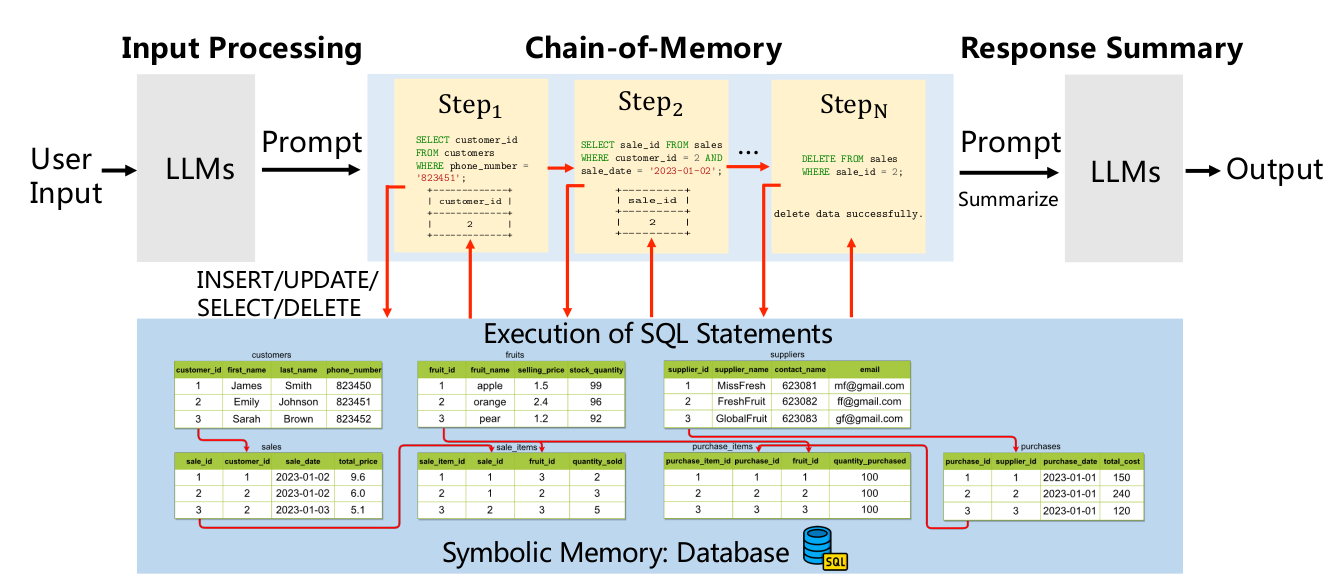
\includegraphics[scale=0.25]{png/process.png}
	\begin{itemize}
		\item input:手机号为823451的顾客在2023年1月2日买了什么东西?
		\item output:买了几个梨
		\item 说明:输入这段话以后,第一步模型尝试从所有顾客中根据手机号823451找出顾客的购物id号,第二步在销售号码中根据顾客的购物id号和购买日期得到销售号,...,通过一步一步有逻辑的推导得到最后的结果具体买了什么水果。
	\end{itemize}
\end{frame}

\section{代码上的工作}

\subsection{构建了一组时间序列的数据集}

\begin{frame}[fragile]
	\frametitle{代码任务的的指令微调数据集示例}	
    \begin{lstlisting}[style=json]
		[
			{
				"instruction": "Write a C++ program that calculates the area of a rectangle, given its width and height.",
				"input": "width: 5, height: 8",
				"response": "#include <iostream>\nusing namespace std;\n\nint main() {\n    int width = 5;\n    int height = 8;\n    int area = width * height;\n\n    cout << \"Area of rectangle: \" << area << endl;\n    return 0;}",
				"output": "#include <iostream>\nusing namespace std;\n\nint main() {\n    int width = 5;\n    int height = 8;\n    int area = width * height;\n\n    cout << \"Area of rectangle: \" << area << endl;\n    return 0;}"
			},
		]
    \end{lstlisting}
	\begin{itemize}
		\item Response(回复):这是指令对应的人工生成的预期输出。回复提供了模型在给定输入下应该生成的参考答案或期望的输出。它可以是文本、图像、标签等,取决于任务的类型。
	\end{itemize}
\end{frame}


\begin{frame}[fragile]
	\frametitle{时间序列预测任务的指令微调数据集示例}	
    \begin{lstlisting}[style=json]
		{
			"Instruction": "For a weather data sequence, from the existing 336 sequences, predict the future 96 sequences?",
			"Input": "2020-01-01 00:10:00,1008.89,0.71,273.18,-1.33,86.1,6.43,5.54,0.89,3.42,5.49,1280.62,1.02,1.6,224.3,0.0,0.0,0.0,0.0,0.0,11.45,428.1,break,2020-01-01 00:20:00,...,0.0,0.0,15.69,56.56,69.3,18.48,425.6,break",
			"output":"425.7,425.9,425.8,...,425.8"
		}
    \end{lstlisting}
	\begin{itemize}
		\item 指令微调数据样例
		\eee{
		\item instruction: "For a \textcolor{red}{weather} data sequence, from the existing \textcolor{red}{336} sequences, predict \textcolor{red}{the temperature indicator} of the future \textcolor{red}{96} sequences ?"
		\item input:"2020-01-01 00:10:00,1008.89,..."(336行21维度的数据)
		\item output:"425.7,425.9,425.8,...,425.8"(96行特定维度的值)
		}
		\item 可以将其中的标红进行修改,来对应不同的数据集.
		\item 问题:输入,输出序列都太长
	\end{itemize}
\end{frame}

% \subsection{时间序列应该怎么修改一下,目前来看这个序列有点简单,要换一种方式,对比一下计算机的代码,然后比较着看}

\subsection{Ptuning代码的参数配置情况}
\begin{frame}[fragile]
    \frametitle{Ptuning运行脚本}

    \begin{lstlisting}[style=shell]
		PRE_SEQ_LEN=128
		LR=2e-2
		
		CUDA_VISIBLE_DEVICES=0 python3 main.py \
			--do_train \ 
			--train_file AdvertiseGen/train.json \
			--validation_file AdvertiseGen/dev.json \
			--prompt_column content \
			--response_column summary \
			--overwrite_cache \
			--model_name_or_path ../chatglm-6b \
			--output_dir output/adgen-chatglm-6b-pt-$PRE_SEQ_LEN-$LR \
			--overwrite_output_dir \
			--max_source_length 64 \
			--max_target_length 64 \
			--per_device_train_batch_size 1 \
			--per_device_eval_batch_size 1 \
			--gradient_accumulation_steps 16 \
			--predict_with_generate \
			--max_steps 3000 \
			--logging_steps 10 \
			--save_steps 1000 \
			--learning_rate $LR \
			--pre_seq_len $PRE_SEQ_LEN \
			--quantization_bit 4				
    \end{lstlisting}
\end{frame}

\begin{frame}
	\frametitle{重要参数}
	\begin{itemize}
		\item PRE\_SEQ\_LEN=128: 这个参数定义了预先截断(pre-truncation)的序列长度。它指定了模型在处理输入和输出序列之前将文本截断或填充到的最大长度。
		\item --max\_source/target\_length\ 64: 这个参数定义了输入/出序列的最大长度。如果输入/出序列超过该长度,将会被截断.
		% \item LR=2e-2: 这个参数定义了学习率
		% (learning rate)即模型在训练过程中更新参数的速度。学习率控制了每次参数更新的步长,较高的学习率可以加快模型的收敛速度,但可能会导致不稳定的训练过程。
		% \item --do\_train: 这是一个命令行选项,表示进行训练。当指定此选项时,模型将进行训练。
		% \item --train\_file AdvertiseGen/train.json: 这个参数指定了训练数据文件的路径。
		% 在这个例子中,训练数据文件是AdvertiseGen/train.json。
		% \item  --validation\_file\ AdvertiseGen/dev.json: 这个参数指定了验证数据文件的路径。
		% 验证数据用于在训练过程中评估模型的性能和选择最佳的模型参数。
		\item --prompt\_column content: 这个参数指定了输入数据中用作指令(prompt)的列。
		% 在这个例子中,输入数据的content列将被用作指令。
		\item --response\_column\ summary: 这个参数指定了输出数据中用作回复(response)的列。
		\item --predict\_with\_generate: 这个参数表示在评估过程中使用生成模式进行预测。在生成模式下,模型将生成回复而不是使用给定的回复
		% 在这个例子中,输出数据的summary列将被用作回复。
		% \item --overwrite\_cache: 这个参数表示是否覆盖缓存。如果指定此选项,缓存文件将被重新生成,否则将使用现有的缓存文件(如果存在)。
		% \item --model\_name\_or\_path ../chatglm-6b: 这个参数指定了使用的预训练模型的名称或路径。
		% 在这个例子中,模型使用了路径../chatglm-6b下的预训练模型。
		% \item --output\_dir\ output/adgen-chatglm-6b-pt-\$PRE\_SEQ\_LEN-\$LR: 这个参数指定了输出目录的路径,用于保存训练过程中的模型和日志文件。在这个例子中,输出目录是output/adgen-chatglm-6b-pt-\$PRE\_SEQ\_LEN-\$LR。
		% \item --overwrite\_output\_dir: 这个参数表示是否覆盖输出目录。如果指定此选项,输出目录将被清空并重新创建,否则将在输出目录中追加生成文件。
		\item --gradient\_accumulation\_steps 16: 这个参数定义了梯度累积的步数。梯度累积可以在训练过程中将多个批次的梯度累积起来,以增加批次大小的效果,从而减少显存的需求。
	\end{itemize}
\end{frame}

\begin{frame}[fragile]
	\frametitle{运行完的结果}	
    \begin{lstlisting}[style=json]
		{
			"epoch": 0.42,
			"train_loss": 4.3601599731445315,
			"train_runtime": 15178.543,
			"train_samples": 114599,
			"train_samples_per_second": 3.162,
			"train_steps_per_second": 0.198
		}
    \end{lstlisting}	
\end{frame}

\subsection{当前遇到的一些问题}
\begin{frame}
	\frametitle{问题}	
	\eee{
		\item 时间序列这个数据集太长了,一般会有一个阶段的长度,所以这边是不是有点问题.对于每个数据向量,能否进行一定的压缩?能否模仿前面论文的方式进行单独存储数据?
		\item 输入数据的方式是否可以改变,接下来打算去看看代码生成繁琐的任务具体是怎么做的?
			% \item ssh chenkejie@10.71.96.8 -p 30002 进不去
		}
\end{frame}

% 结束语
\section{}
\begin{frame}
	\frametitle{}
	\begin{center}
		\Huge{谢谢老师和同学的聆听!}
	\end{center}
\end{frame}


\end{CJK*}
\end{document}